\section{Security}

\subsection{Generic security requirements}

\begin{itemize}
		\item Traditional: Confidentiality, authenticity, integrity, (operational security)
		\item Based on these: Access control, non-repudiation, dependability, safety, privacy
\end{itemize}

\subsection{Threats in IoT}

\begin{itemize}
		\item Passive information gathering, replay attacks
		\item Captured nodes, malicious nodes
		\item DoS of network, memory, CPU, energy at various layers
\end{itemize}

\subsection{Requirements for IoT}

\begin{itemize}
		\item Data confidentiality, authenticity, integrity
		\item Freshness: Keys should be refreshed, data should be fresh (not replay attack)
		\item Availability: Survivability to DOS at various layers
\end{itemize}

\subsection{Crypto 101}

\begin{description}
		\item[Encryption] Transforming plaintext into ciphertext using (keyed)
				algorithm.
		\item[Decryption] Reverse of encryption
		\item[Symmetric encryption] Sender and receiver share same key, eg
				block ciphers DES/AES, stream ciphers OTP.
		\item[Asymmetric encryption] Public key for encryption, private for
				decryption. Eg RSA, DSA, ElGamal.
\end{description}

\subsection{Approaches for IoT}

\begin{description}
		\item[Single network-wide key] Low overhead, but compromise of a single
				node compromises whole network
		\item[Pairwise keys] Easy revocation of keys of one node possible, poor scalability.
		\item[Asymmetric cryptography] Scalable, but computationally expensive.
				Vulnerable to DoS.
\end{description}

\subsection{Security properties of IoT systems}

\begin{itemize}
		\item Asymmetric crypto very expensive, especially on low-power nodes.
		\item Lack of central control
		\item Error-prone communication, hard to distinguish fault from attack
		\item No global identification, IDs of nodes might be stolen
		\item Hostile environment, nodes have little physical protection
		\item In-network processing (aggregation etc)
		\item IoT OS will provide limited safety measures compared to full OS
		\item OTA updates are risky and potentially unsecure
		\item WIFI security flaws, hardware backdoors (management interfaces),
				only partial certificate verification, ...
\end{itemize}

\subsection{Cell-based WSN}

\begin{itemize}
		\item Can use base station as trust anchor
		\item Base station can (and must) implement access control
		\item Example: SPINS protocol suite, contains `Sensor network
				encryption protocol' (SNEP) for secure unicast communication
				between base station and nodes. Provides confidentiality,
				two-party authentication, integrity, freshness.
\end{itemize}

\subsubsection{SPINS}

\paragraph{Assumptions}

\begin{itemize}
		\item Base stations have sufficient battery and processing power
		\item Nodes send readings to base station, base station sends requests, queries and reprogramming to nodes
\end{itemize}

\paragraph{Notation}

\begin{description}
		\item[$A, B$] Communication principals such as nodes
		\item[$N_A$] generated by $A$
		\item[$X_{AB}$] Shared master key between $A$, $B$, used to key PRF
		\item[$F$] PRF
		\item[$K_{AB}$, $K_{BA}$] Encryption keys, $K_{AB} = F_{X_{AB}}(1), K_{BA} = F_{X_{AB}}(3)$
		\item[$K'_{AB}$, $K'_{BA}$] MAC keys, $K'_{AB} = F_{X_{AB}}(2), K'_{BA} = F_{X_{AB}}(4)$
		\item[$\{M\}_{K_{AB}, IV}$] Message $M$ encrypted with $K_{AB}$ and initialization vector $IV$
		\item[$MAC(K'_{AB}, M)$] MAC of message $M$ with key $K'_{AB}$
		\item[$C_A$] Counter at $A$
\end{description}

\paragraph{SNEP}

SNEP messages combine:
\begin{itemize}
		\item Encryption with encryption keys $K_{AB}, K_{BA}$
		\item Authentication with MAC keys $K'_{AB}, K'_{BA}$
		\item Messages from $A$ to $B$ contain $\{D\}_{K_{AB}, C_A}$ and $MAC(K'_{AB}, C_A || \{D\}_{K_{AB}, C_A}$
		\item Hence offers semantic security, data authentication, replay protection, weak freshness, low overhead
		\item Rather than truly random IV, use synchronized counters for replay
				protection. Problem: Packet loss, so counters must be
				synchronized.
\end{itemize}

\paragraph{SNEP counter exchange protocols}

Counters are non-private, so no need for encryption, but must be fresh. Initial
bootstrapping:

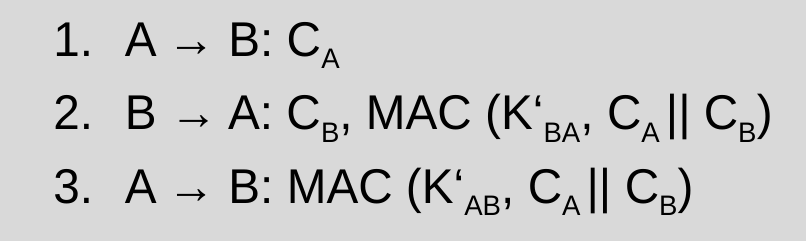
\includegraphics[width=0.5\textwidth]{11_snep_cep_bootstrap}

And sync whenever node detects that other's counter out of sync:

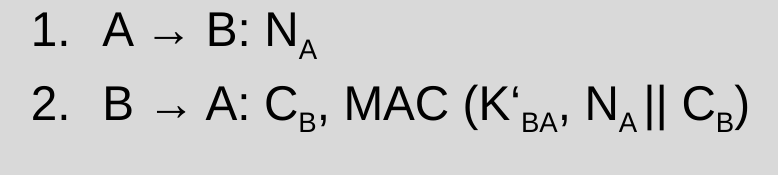
\includegraphics[width=0.5\textwidth]{11_snep_cep_sync}


\subsubsection{uTesla}

Idea: Allow authenticated broadcast using symmetric keys, disclosure of which
is delayed.

\begin{enumerate}
		\item Packet transmission: Base station broadcasts message with MAC
				using secret symmetric key
		\item Packet reception: Receivers detect (loosely synchronized clock)
				that authentication key for this packet missing
		\item Key disclosure: Base station broadcasts key to all receivers,
				which then verify packet
\end{enumerate}

\paragraph{Authentication key calculation}

\begin{itemize}
		\item Sender chooses key $K_n$, applies one-way function $F$ to all other keys $K_{i-1} := F(K_{i})$
		\item Time divided into intervals, usage of a single key $K_i$ during time interval $i$
		\item Once key $K_{i+1}$ disclosed, all keys $K_0 \ldots K_i$ can be
				reconstructed, allows nodes to reconstruct keys they might have
				missed
		\item Keys disclosed after certain interval $\delta$
		\item Receivers can \textbf{also} verify $K_{i+1} == F(K_i)$, so can
				verify that newly released key is legit. Self-authenticating
				keys. But requires receiver to know one key in the chain.
\end{itemize}

\paragraph{Security considerations}

\begin{itemize}
		\item Only packets received while key not yet disclosed are to be trusted
		\item Packets received after key was disclosed might be forged
		\item Receiver must know disclosure schedule $(T_i, T_{int}, \delta)$
\end{itemize}

\paragraph{Key disclosure scheme}

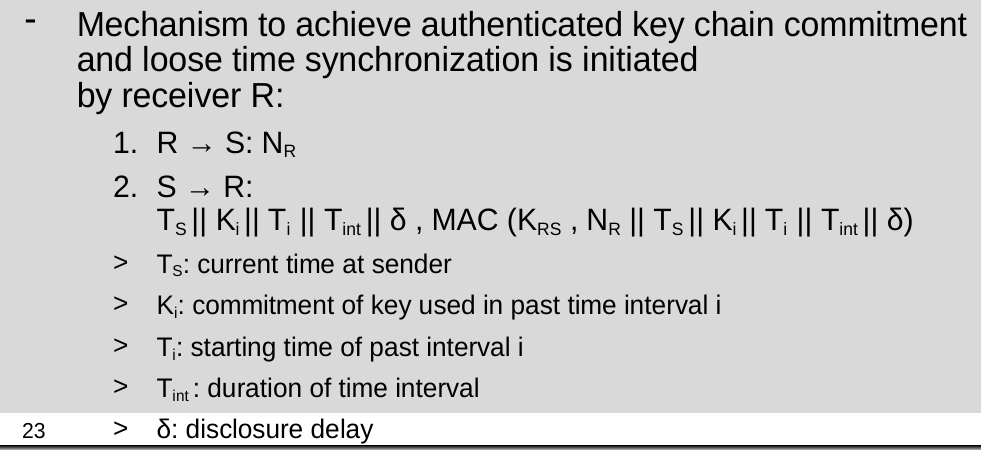
\includegraphics[width=0.5\textwidth]{11_utesla}

\subsubsection{TinySec}

\begin{itemize}
		\item Lightweight, MAC for each packet
		\item IV must be long enough to prevent conflict, short enough to be feasible
		\item CBC encryption reuses block cipher for MAC
		\item No replay protection, that one done by application layer (if required)
\end{itemize}

\subsubsection{Localized encryption and authentication protocol, LEAP+}

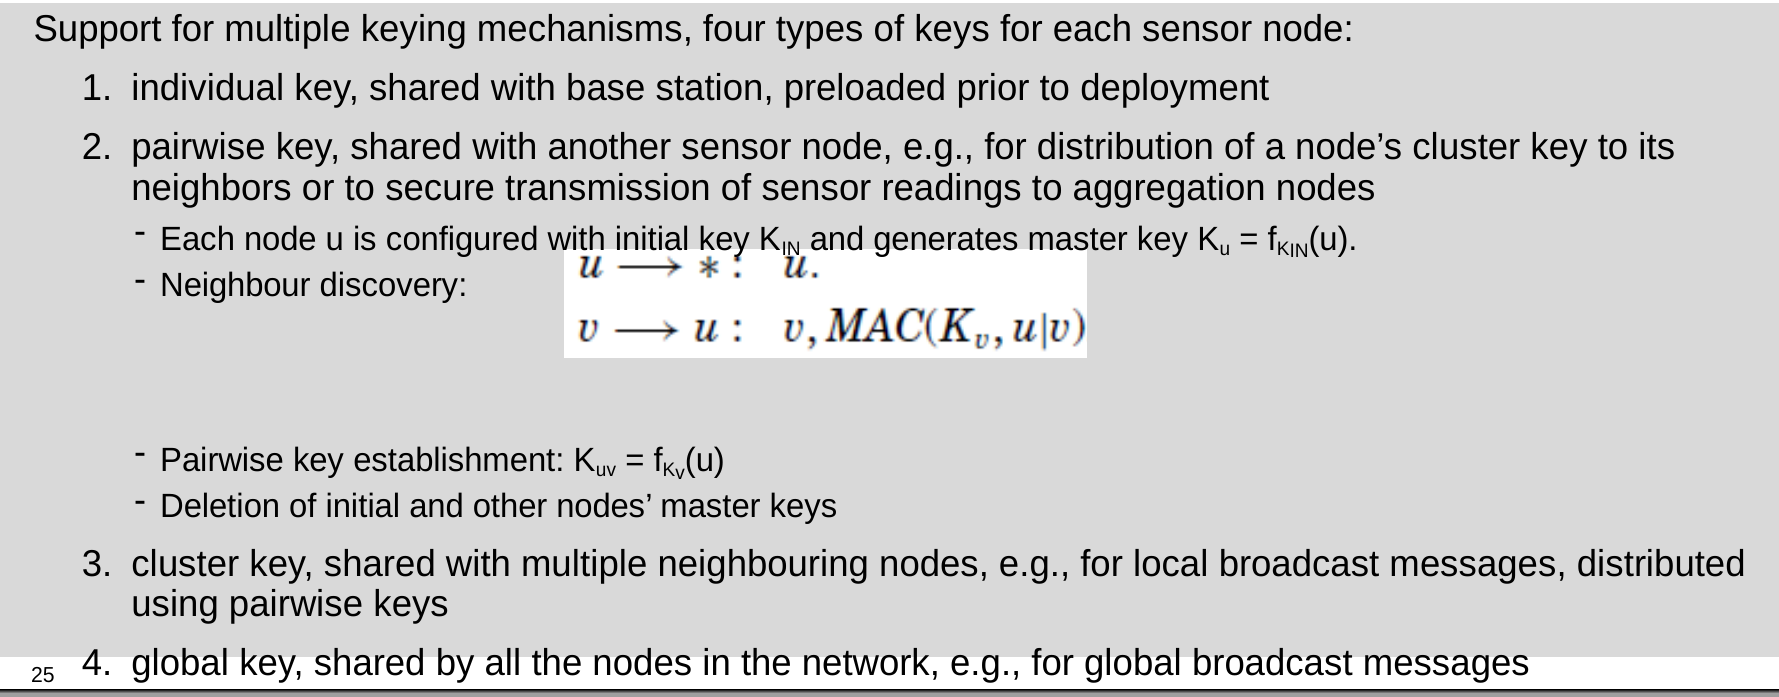
\includegraphics[width=\textwidth]{11_leap}

\subsubsection{IEEE 802.15.4 and ZigBee}

\begin{itemize}
		\item Basic security models, eg access control, integrity, confidentiality, replay protection
		\item Security by MAC layer
		\item 8 standard security modes, CTR, CBC, ...
		\item Trusted coordinator responsible for key distribution
\end{itemize}

\subsection{Ad Hoc networks}

\begin{itemize}
		\item Prefer symmetric keys, \textbf{no trusted base station}
		\item Typically based on pre-deployed keys, be it one for whole network
				(can be compromised), one for each keypair (does not scale), or
				probabilistic (shared between $x$ nodes)
\end{itemize}

\subsubsection{Probabilistic key distribution}

\begin{itemize}
		\item Generation of pool of $P$ keys pre-deployment
		\item $k < P$ keys installed on each node, where eg $k = 250, P = 100000$
		\item Compromised node exposes $k / P$ of total keys.
		\item Two nodes exchange information about available keys. Birthday paradox makes it quite likely that at least one common key
		\item Shared keys establish topology. If two nodes not connected, they have to establish a path
\end{itemize}

\paragraph{Path-key establishment}

\begin{itemize}
		\item Idea: Establish path via intermediary nodes
		\item Problem: intermediate nodes now nkow key
		\item Solution: Secret sharing, establish key as combination of
				components shared via disjoint paths, $k = k_1 \oplus k_2
				\oplus ... \oplus k_n$
		\item Problem: Finding disjoint paths
\end{itemize}

\subsection{Denial of service attacks}

\subsubsection{On phsyical layer}

\begin{itemize}
		\item Tampering with nodes
		\item Jamming of signal: Constant (noise), random (noise), decepting (packet injection), reactive (when node detected as active)
\end{itemize}

\paragraph{Detecting jamming}

\begin{description}
		\item[Signal strength] Reactive jammer and active node look alike
		\item[Carrier sensing time] Reactive or random jammer hard to detect
		\item[Packet delivery ratio] Quality can also be low for legit traffic
		\item[Combination of signal strength and packet delivery ratio] High
				strength and low delivery ratio might indicate jamming
\end{description}

\paragraph{Defending}

\begin{itemize}
		\item Frequency hopping
		\item Error-correcting codes
		\item Rerouting around jamming regions
\end{itemize}

\subsubsection{On link layer}

\begin{itemize}
		\item Fabricated collisions (checksum mismatch): Employ ECC
		\item Exhaustion (ask for retransmissions): Nodes should limit retransmission frequency
		\item Unfariness (abuse cooperative layer)
\end{itemize}

\subsubsection{On routing layer}

\begin{itemize}
		\item Neglect routing: Redundant routes
		\item Sybil attack: Pairwise frequency hopping between nodes
		\item Attacks on special nodse (e.g. cluster heads): Hide node locations
		\item Cause incorrect routing: Monitor and authenticate routing advertisements
		\item Black hole traffic: Probe and reroute
		\item Replaying traffic in other part of network: Timestamp / add location to messages
\end{itemize}

\subsusbection{On transport layer}

\begin{itemize}
		\item Flooding: Clients must solve puzzle (proof-of-work) before initiating connection
		\item Desynchronization (attacker sends wrong state information to
				cause retransmissions): Authenticated control message
\end{itemize}
